\documentclass[10pt]{article}
\usepackage[utf8]{inputenc}
\usepackage[T1]{fontenc}
\usepackage{amsmath}
\usepackage{amsfonts}
\usepackage{amssymb}
\usepackage[version=4]{mhchem}
\usepackage{stmaryrd}
\usepackage{graphicx}
\usepackage[export]{adjustbox}
\graphicspath{ {./images/} }
\usepackage{bbold}

\title{Probability and Statistics \\
 Statistics }

\author{Giuliano Casale\\
Department of Computing, Imperial College London}
\date{}


\begin{document}
\maketitle


% \section*{Statistics versus Probability}
% "Arrivals to a web server have exponential inter-arrival times with rate $\lambda=0.2$ jobs $/$ second. Determine the probability that the next job arrives in less than 1 second." $\Rightarrow$ Typical probability question\\
% "In a period of one hour, you collect observations of the interarrival times of jobs. Estimate the parameter $\lambda$ for the exponential distribution that best fits the data."\\
% $\Rightarrow$ Typical statistics question (estimation)\\
% "After some time, you suspect the arrivals have changed distribution. Is there a strong evidence that $\lambda \neq 0.2$ ?"\\
% $\Rightarrow$ Typical statistics question (hypothesis testing)\\
% Statistics studies how to infer properties of the distribution underlying data we observe.

% \section*{Statistical Modelling}
% Statistics assumes the availability of a sample of observations.

% \begin{itemize}
%   \item A sample is a subset of a population of interest for the study.
%   \item e.g., a voting poll uses a random sample of the voters.
% \end{itemize}

% We focus on parametric statistics, where the population's data follow some distribution, e.g.: $\operatorname{Exp}(\lambda), \mathrm{N}\left(\mu, \sigma^{2}\right)$, etc.

% The goal is then to estimate the model parameters ( $\lambda, \mu, \sigma^{2}, \ldots$ ) from the sample of observed data.

% \begin{itemize}
%   \item Samples will be affected by uncertainty due to limited sample size and due to the random selection.
% \end{itemize}

% \section*{Estimation Theory}
% \section*{Definitions}
% \begin{itemize}
%   \item A sample of data $x=\left(x_{1}, \ldots, x_{n}\right)$, may be seen as a realisation of a set of random variables $X=\left(X_{1}, \ldots, X_{n}\right)$.
%   \item We assume that a single draw $X_{i}$ follows a distribution
% \end{itemize}

% $$
% P(\cdot \mid \theta)
% $$

% where $\theta=\left(\theta_{1}, \ldots, \theta_{r}\right)$ are parameters we wish to estimate.

% \begin{itemize}
%   \item We will assume that our $n$ data point random variables $X$ are independent and identically distributed (i.i.d.).
%   \item The last assumption implies that sampling is with replacement, thus any number of samples $n$ may be collected.
% \end{itemize}

% \section*{Estimator is a Statistic}
% \begin{itemize}
%   \item A statistic is a function of the random sample
% \end{itemize}

% $$
% T=T(X)=T\left(X_{1}, \ldots, X_{n}\right)
% $$

% and is itself a random variable.

% \begin{itemize}
%   \item If a statistic $T(X)$ is used to approximate parameters in $\theta$, we say that $T$ is an estimator for those parameters.
%   \item The actual realisation $t(x)$ of the estimator for a particular data sample $x$ is called an estimate of the parameter(s).
%   \item Example: $\bar{X}=S_{n} / n=\sum_{i=1}^{n} X_{i} / n$ is the sample mean statistic. Its realization $\bar{x}=\sum_{i=1}^{n} x_{i} / n$ is an estimate.
%   \item In what follows, we will study the sampling distribution for the statistic, i.e., $P(T \mid \theta) \equiv P(T(X) \mid \theta)$, and its moments.
% \end{itemize}

% \section*{Example: Estimators for the Mean}
% \begin{itemize}
%   \item Consider a sample $\left(X_{1}, \ldots, X_{n}\right)$ where $X_{i} \sim \operatorname{Exp}(\lambda)$ distribution, $\forall i$, for which $\lambda$ is unknown.
%   \item We might construct estimators for either $\lambda$, for the mean of the distribution ( $\mu=\lambda^{-1}$ ), or for the variance ( $\sigma^{2}=\lambda^{-2}$ ).
%   \item For the mean, we could propose as estimator:
%   \item the first value we have observed, i.e., $T(X)=X_{1}$
%   \item or the sample mean $T(X)=\bar{X}$
%   \item or the median $T(X)=\operatorname{med}(X)$
%   \item Q: How would you choose which estimator is better?
% \end{itemize}

% \section*{Bias of Estimator}
% \begin{itemize}
%   \item We define the bias of an estimator $T$ for a parameter $\theta$ as
% \end{itemize}

% $$
% \operatorname{bias}(T)=E(T \mid \theta)-\theta .
% $$

% \begin{itemize}
%   \item This requires to determine the expectation of $T(X)$ based on the sampling distribution.
%   \item If the estimator has zero bias we say it is unbiased.
%   \item For example, $\bar{X}=\frac{1}{n} \sum_{i=1}^{n} X_{i}$ gives an unbiased estimate of the mean of an exponential distribution (which is $\mu=\lambda^{-1}$ ).
%   \item This is true for any distribution: the sample mean $\bar{X}$ is an unbiased estimate for the population mean $\mu$
% \end{itemize}

% $$
% E(\bar{X})=E\left(\frac{\sum_{i=1}^{n} X_{i}}{n}\right)=\frac{\sum_{i=1}^{n} E\left(X_{i}\right)}{n}=\frac{n \mu}{n}=\mu .
% $$

% \section*{Sample Variance}
% How can we obtain an unbiased estimator for the variance?

% Let $X_{1}, \ldots, X_{n}$ be i.i.d. random variables, each with mean $\mu$ and variance $\sigma^{2}$. We may be tempted to consider the sample variance

% $$
% \frac{1}{n} \sum_{i=1}^{n}\left(X_{i}-\bar{X}\right)^{2}
% $$

% Unfortunately, it can be shown that this is biased. Only, if we know the population mean $\mu$, then $\frac{1}{n} \sum_{i=1}^{n}\left(X_{i}-\mu\right)^{2}$ is unbiased for $\sigma^{2}$.

% \section*{Bias-Corrected Sample Variance}
% The random variable $S^{2}$ defined by


% \begin{equation*}
% S^{2}=\frac{1}{n-1} \sum_{i=1}^{n}\left(X_{i}-\bar{X}\right)^{2} \tag{1}
% \end{equation*}


% is called the bias-corrected sample variance of these data. The $\frac{1}{n-1}$ term, also referred to as Bessel's correction, ensures that $S$ is an unbiased estimator, i.e. $E\left[S^{2}\right]=\sigma^{2}$.

% \section*{Proof: Bessel's correction}
% We first note the following identity

% $$
% \begin{aligned}
% \sum_{i=1}^{n}\left(X_{i}-\bar{X}\right)^{2} & =\sum_{i=1}^{n}\left(X_{i}-\mu+\mu-\bar{X}\right)^{2} \\
% & =\sum_{i=1}^{n}\left(X_{i}-\mu\right)^{2}+n(\mu-\bar{X})^{2}+2 \sum_{i=1}^{n}(\mu-\bar{X})\left(X_{i}-\mu\right) \\
% & =\sum_{i=1}^{n}\left(X_{i}-\mu\right)^{2}+n(\mu-\bar{X})^{2}+2(\mu-\bar{X})(n \bar{X}-n \mu) \\
% & =\sum_{i=1}^{n}\left(X_{i}-\mu\right)^{2}+n(\mu-\bar{X})^{2}-2 n(\mu-\bar{X})^{2} \\
% & =\sum_{i=1}^{n}\left(X_{i}-\mu\right)^{2}-n(\bar{X}-\mu)^{2}
% \end{aligned}
% $$

% \section*{Proof: Bessel's correction}
% Using the identity we just found, we get

% $$
% \begin{aligned}
% E\left[(n-1) S^{2}\right] & =\sum_{i=1}^{n} E\left[\left(X_{i}-\mu\right)^{2}\right]-n E\left[(\bar{X}-\mu)^{2}\right] \\
% & =n \sigma^{2}-n \operatorname{Var}(\bar{X})=(n-1) \sigma^{2}
% \end{aligned}
% $$

% where we have used that $\operatorname{Var}(\bar{X})=\operatorname{Var}\left(S_{n} / n\right)=\sigma^{2} / n$.\\
% Since $n$ is a scalar, $E\left[(n-1) S^{2}\right]=(n-1) E\left[S^{2}\right]$, hence the result implies that for the bias-corrected sample variance

% $$
% E\left[S^{2}\right]=\sigma^{2}
% $$

% \section*{Efficiency of Estimators}
% \begin{itemize}
%   \item Suppose we have two unbiased estimators for a parameter $\theta$, which we will call $T \equiv T(X)$ and $H \equiv H(X)$.
%   \item Suppose that we know the corresponding sampling distributions, $P(T \mid \theta)$ and $P(H \mid \theta)$, so that we can calculate their variances.
%   \item We say $T$ is more efficient than $H$ if
%   \item $\forall \theta \quad \operatorname{Var}(T \mid \theta) \leq \operatorname{Var}(H \mid \theta)$
%   \item $\exists \theta \quad \operatorname{Var}(T \mid \theta)<\operatorname{Var}(H \mid \theta)$.
%   \item If $T$ is more efficient than any other possible estimator, we say that $T$ is efficient.
% \end{itemize}

% \section*{Example: Bias \& Efficiency}
% \begin{itemize}
%   \item Suppose we have a population with mean $\mu$ and variance $\sigma^{2}$. Now, consider two estimators for $\mu$
%   \item the sample mean $T=\bar{X}$
%   \item the first observation in the sample $H=X_{1}$
%   \item We have seen that always $E(\bar{X})=\mu$, and certainly $E\left(X_{1}\right)=\mu$, so both estimators are unbiased.
%   \item We also know
% \end{itemize}

% $$
% \operatorname{Var}(\bar{X})=\frac{\sigma^{2}}{n} \quad \text { and } \quad \operatorname{Var}\left(X_{1}\right)=\sigma^{2}
% $$

% \begin{itemize}
%   \item So for $n \geq 2, T$ is more efficient than $H$ as an estimator of $\mu$.
% \end{itemize}

% \section*{Consistency of Estimators}
% \begin{itemize}
%   \item In the last example, the worst aspect of the estimate $H=X_{1}$ is that it does not improve as $n$ increases.
%   \item Consistency allows us to recognize behaviours such as this as $n$ grows large.
%   \item We say $T$ is a consistent estimator for the parameter $\theta$ if
% \end{itemize}

% $$
% \forall \varepsilon>0, \quad P(|T(X)-\theta|>\varepsilon) \rightarrow 0 \text { as } n \rightarrow \infty
% $$

% In other words, all probability mass of the estimator (seen as a random variable) is asymptotically on the value $\theta$.

% \begin{itemize}
%   \item If $T$ is unbiased and the condition $\lim _{n \rightarrow \infty} \operatorname{Var}(T(X))=0$ holds, this is sufficient to show that $T$ is consistent.
%   \item In our example, we get that $\bar{X}$ is a consistent estimator of $\mu$, while $X_{1}$ is not since its variance is constant for all $n$. Instead, $\bar{X}+\frac{1}{n}$ is biased but consistent.
% \end{itemize}

\section*{Maximum Likelihood Estimation}
\section*{Example: Likelihood for Continuous Distributions}
We need to build a reliability model for disk drives in a data center. Let us assume that the time to failure of a disk drive follows an exponential distribution, with density $f(x)=\lambda e^{-\lambda x}$, where $x$ is the time to failure.

We record the following failure times for 10 disks, in hours:\\
$X=\left(x_{i}\right)=(1200,1500,1600,1700,1100,1300,1400,1250,1550,1650)$\\
How can we best choose $\lambda$ ?\\

\includegraphics[max width=\textwidth, center]{2025_05_12_2c033a5f0417cd8b136fg-17}

\section*{Example: Likelihood for Continuous Random Variables}
Idea: We seek for the $\lambda$ value that maximizes the chances of sampling what we observed.\\
For a continuous distribution, we may do so by choosing $\lambda$ that maximizes the joint pdf:

$$
L(\lambda)=f(X \mid \lambda)=f\left(x_{1}, \ldots, x_{10} \mid \lambda\right)=\prod_{i=1}^{10} f\left(x_{i} \mid \lambda\right)=\prod_{i=1}^{10} \lambda e^{-\lambda x_{i}}
$$

where we used independence.\\
Finally, we use basic calculus to find the $\lambda$ that maximizes $f(X \mid \lambda)$ :

$$
\widehat{\lambda}=\arg \max _{\lambda} L(\lambda)=\frac{10}{\sum_{i=1}^{n} x_{i}}=\frac{1}{\bar{X}}=\frac{1}{1425}=0.0007 \text { failures } / \mathrm{h}
$$

where $\bar{X}$ is the observed mean time to failure (MTTF).

\section*{Example: Log-Likelihood for Continuous Distributions}
To prove the last result, it is easier to work with the logarithm of $L(\lambda)$, which we refer to as the log-likelihood

$$
\ell(\lambda)=\log L(\lambda)=\log \prod_{i=1}^{n} \lambda e^{-\lambda x_{i}}=n \log \lambda-\lambda \sum_{i=1}^{n} x_{i}
$$

Since the logarithm is monotone, we can equivalently maximize $\ell(\lambda)$ instead of $L(\lambda)$. In this case, the maximum is found by setting

$$
\ell^{\prime}(\lambda)=\frac{d}{d \lambda} \ell(\lambda)=\frac{n}{\lambda}-\sum_{i=1}^{n} x_{i}=0
$$

that yields $\widehat{\lambda}=\frac{n}{\sum_{i=1}^{n} x_{i}}=\frac{1}{\bar{x}}$. Since $\ell^{\prime \prime}(\widehat{\lambda})<0$, this is a maximum.

\section*{Example: Likelihood for Discrete Distributions}
\begin{itemize}
  \item Let us now assume a discrete setting, where we count every day the number of disks $x$ that fail. The data center has $m=20000$ disks.
  \item Over the last $d=100$ days, we observe the following data:
\end{itemize}

\begin{center}
\begin{tabular}{|l|c|c|c|c|c|c|c|c|c|c|c|}
$x$ & 0 & 1 & 2 & 3 & 4 & 5 & 6 & 7 & 8 & 9 & 10 \\
\hline
Frequency & 2 & 16 & 35 & 22 & 21 & 3 & 1 & 0 & 0 & 0 & 0 \\
\hline
\end{tabular}
\end{center}

\begin{itemize}
  \item Assuming that disks are independent, we treat our dataset as a sample of $\operatorname{Binomial}(m, \theta)$ with $p(x \mid \theta)=\binom{m}{x} \theta^{x}(1-\theta)^{m-x}$, where $\theta$ is the (daily) disk failure probability.
  \item How shall we estimate $\theta$ ?
\end{itemize}

\section*{Example: Likelihood for Discrete Distributions}
Idea: again, we seek for the $\theta$ value that maximizes the chances of sampling what we observed.\\
For a discrete distribution, we model this using the joint pmf:

$$
L(\theta)=p\left(x_{1}, \ldots, x_{d} \mid \theta\right)=\prod_{i=1}^{d}\binom{m}{x_{i}} \theta^{x_{i}}(1-\theta)^{m-x_{i}}
$$

where the last passage follows again from independence.\\
Lastly, we find the $\theta$ that maximizes $L(\theta)$, which is

$$
\widehat{\theta}=\arg \max _{\theta} L(\theta)=\frac{1}{d} \frac{\sum_{i=1}^{d} x_{i}}{m}=0.0001285 \text { failure probability }
$$

(Left to check as an exercise.)

\section*{Maximum Likelihood Estimation}
(1) The likelihood function, $L(\theta)=\prod_{i=1}^{n} f\left(x_{i} \mid \theta\right)$ is the product of the $n \mathrm{pmf} / \mathrm{pdf}$ viewed as a function of a parameter $\theta$.\\
(2) Take the natural log of the likelihood to get the log-likelihood function $\ell(\hat{\theta})=\log (L(\theta))$ and collect terms involving $\theta$.\\
(3) Find the value of $\theta$ for which $\log$-likelihood is maximised. This is typically done by finding $\hat{\theta}$ that solves

$$
\ell^{\prime}(\hat{\theta})=\frac{d}{d \theta} \log (L(\hat{\theta}))=0
$$

(1) If the estimate $\hat{\theta}$ obtained in step 3 corresponds to a maximum $\frac{d^{2}}{d \theta^{2}} \ell(\hat{\theta})<0$, then $\hat{\theta}$ is confirmed as the maximum likelihood estimator (MLE) of $\theta$.

\section*{Further remarks on MLE}
\begin{itemize}
  \item In large sample sizes, the MLE progressively becomes unbiased, efficient and consistent. This can be proved under mild technical assumptions.
  \item In small sample sizes there is no such guarantee and the quality of a MLE can vary. Bayesian parameter estimation is an area of statistics that deals with this problem.
  \item For single parameter MLE, if $\theta$ is discrete and $\ell(\cdot)$ unimodal, then we can run MLE as usual, compare $\lceil\hat{\theta}\rceil$ and $\lfloor\hat{\theta}\rfloor$, and return the one having the largest likelihood. Otherwise, more complex algorithms are required to search for the MLE.
  \item MLE generalizes to multi-parameter distributions. Yet this requires multivariate calculus and the maximization may give more than one answer if $\ell$ has several peaks (local maxima).
\end{itemize}

\section*{An alternative to MLE: the method of moments}
\begin{itemize}
  \item In some cases, we may only know statistics of a distribution, such as its sample mean or sample variance.
  \item In this setting, MLE is not viable but we can still estimate parameters if we have enough sample moments.
  \item This approach, called moment matching (or method of moments), tries to match the true and sample moments.
  \item For example, in the disk drive reliability model we had
\end{itemize}

$$
\lambda=\frac{1}{E[X]} \quad \bar{X}=1425
$$

and matching $E[X]=\bar{X}$ yields $\lambda=1 / \bar{X}=1 / 1425=0.0007$.

\begin{itemize}
  \item This is effective on simple models, but unlike MLE can suffer biases for more complex distributions.
\end{itemize}

\section*{Central Limit Theorem}
\section*{The Central Limit Theorem (CLT)}
The CLT is a general result for sums of random variables. In statistics, it helps to study the distribution of the sample mean.

Let $X_{1}, X_{2}, \ldots, X_{n}$ be now $n$ independent and identically distributed (i.i.d.) random variables from any probability distribution with mean $\mu$ and variance $\sigma^{2}$ both finite.

\begin{itemize}
  \item We know that $\mathrm{E}\left(S_{n}\right)=n \mu$ and $\operatorname{Var}\left(S_{n}\right)=n \sigma^{2}$.
  \item Thus, we have $\mathrm{E}\left(S_{n}-n \mu\right)=0$ and $\operatorname{Var}\left(S_{n}-n \mu\right)=n \sigma^{2}$.
  \item Dividing by $\sqrt{n} \sigma$,
\end{itemize}

$$
\mathrm{E}\left(\frac{S_{n}-n \mu}{\sqrt{n} \sigma}\right)=0, \quad \operatorname{Var}\left(\frac{S_{n}-n \mu}{\sqrt{n} \sigma}\right)=1
$$

However, what can we say about the underlying distribution?

We have the following celebrated result:

\section*{Central Limit Theorem (CLT)}
$$
\lim _{n \rightarrow \infty} \frac{S_{n}-n \mu}{\sqrt{n} \sigma} \sim \mathrm{~N}(0,1)
$$

This result can also be written as

$$
\lim _{n \rightarrow \infty} \frac{\bar{X}-\mu}{\sigma / \sqrt{n}} \sim \mathrm{~N}(0,1)
$$

where $\bar{X}=\frac{S_{n}}{n}=\frac{\sum_{i=1}^{n} X_{i}}{n}$ is the sample mean.

\section*{Implications for the Sample Mean}
The CLT thus implies that for large, but finite, $n$

$$
\bar{X} \approx \mathrm{~N}\left(\mu, \frac{\sigma^{2}}{n}\right)
$$

\begin{itemize}
  \item A rule of thumb for "large $n$ " is often $n \geq 30$.
  \item Amazingly, this result holds irrespective of the distribution of the $\left\{X_{i}\right\}$ (and including discrete random variables). CLT thus demonstrates that statistical regularity can arise even from the combination of highly-diverse random phenomena.
  \item If $X_{i} \sim \mathrm{~N}\left(\mu, \sigma^{2}\right), \forall i$, the result becomes exact even for finite $n$, since the sum of independent normal random variables is normally distributed (proof via mgfs).
\end{itemize}

\section*{Sketch proof of the CLT}
Given the $n$ i.i.d. r.vs. $X_{1}, X_{2}, \ldots, X_{n}$, standardise their sum to get

$$
Z_{n}=\frac{S_{n}-n \mu}{\sqrt{n \sigma^{2}}}=\frac{\sum_{i=1}^{n} X_{i}-n \mu}{\sqrt{n \sigma^{2}}}=\frac{\sum_{i=1}^{n}\left(X_{i}-\mu\right)}{\sqrt{n} \sigma}=\sum_{i=1}^{n} \frac{Y_{i}}{\sqrt{n} \sigma}
$$

where $Y_{i}=X_{i}-\mu$ is a shifted version of $X_{i}$ with zero mean.\\
The moment generating function (mgf) of $Z_{n}$ is

$$
M_{Z_{n}}(t)=\left(M_{Y}\left(\frac{t}{\sqrt{n} \sigma}\right)\right)^{n}
$$

where $M_{Y}$ is the mgf of $Y_{1}$ (and each $Y_{i}$ ).

\begin{itemize}
  \item We can now expand $M_{Y}(t)$ at zero using Taylor's theorem
\end{itemize}

$$
M_{Y}(t)=M_{Y}(0)+M_{Y}^{\prime}(0) t+\frac{1}{2} M_{Y}^{\prime \prime}(0) t^{2}+O\left(t^{3}\right)=1+\frac{1}{2} \sigma^{2} t^{2}+O\left(t^{3}\right)
$$

where we note that the derivatives of the mgf are:\\
$M_{Y}^{\prime}(0)=E\left(Y_{i}\right)=0$ and\\
$M_{Y}^{\prime \prime}(0)=E\left(Y_{i}^{2}\right)=\sigma^{2}+E\left(Y_{i}\right)^{2}=\sigma^{2}$.

\begin{itemize}
  \item Plugging the result back into $M_{Z_{n}}(t)$, we can see that
\end{itemize}

$$
\lim _{n \rightarrow+\infty} M_{Z_{n}}(t)=\lim _{n \rightarrow+\infty}\left(1+\frac{t^{2}}{2 n}+O\left(n^{-3 / 2}\right)\right)^{n} \rightarrow e^{t^{2} / 2}
$$

\begin{itemize}
  \item But $e^{t^{2} / 2}$ is the mgf of the standard Normal distribution.
\end{itemize}

\section*{Application to coin tossing}
Consider the simplest example, where $X_{1}, X_{2}, \ldots$ are i.i.d. Bernoulli $(p)$ discrete random variables taking values 0 or 1 .

\begin{itemize}
  \item Then the $\left\{X_{i}\right\}$ have mean $\mu=p$ and variance $\sigma^{2}=p(1-p)$.
  \item Thus, by definition, for any $n$,
\end{itemize}

$$
\sum_{i=1}^{n} X_{i} \sim \operatorname{Binomial}(n, p)
$$

which has mean $n p$ and variance $n p(1-p)$.

\begin{itemize}
  \item But now, by the CLT
\end{itemize}

$$
\operatorname{Binomial}(n, p) \approx \mathrm{N}\left(n \mu, n \sigma^{2}\right) \equiv \mathrm{N}(n p, n p(1-p))
$$

\section*{Binomial $\left(10, \frac{1}{2}\right)$ pmf \& N(5,2.5) pdf}
\begin{center}
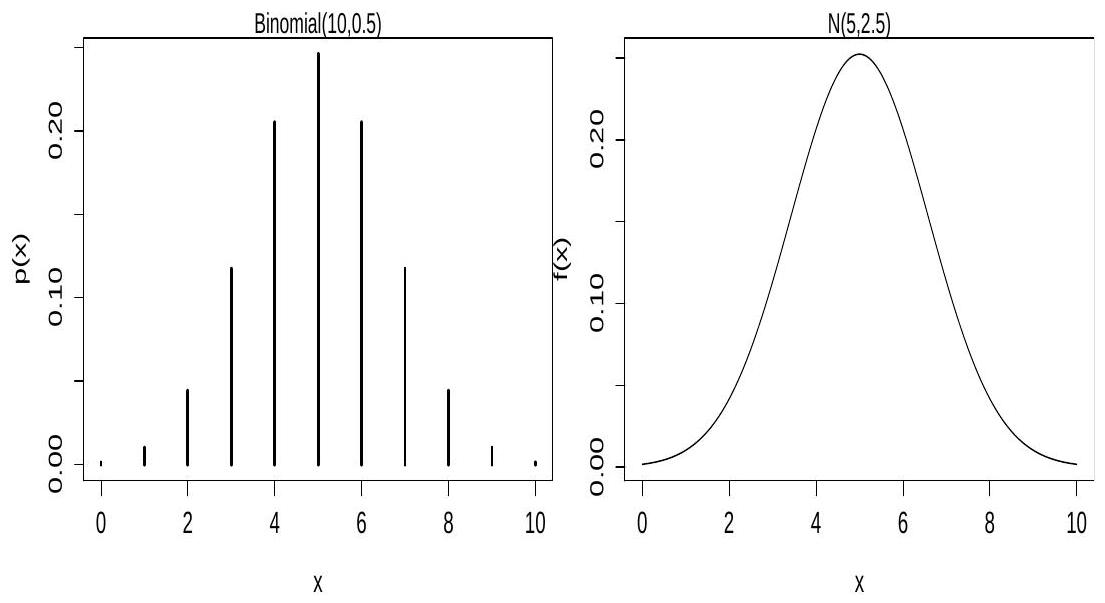
\includegraphics[max width=\textwidth]{2025_05_12_2c033a5f0417cd8b136fg-32}
\end{center}

\section*{Binomial $\left(100, \frac{1}{2}\right)$ pmf \& N $(50,25)$ pdf}
\begin{center}
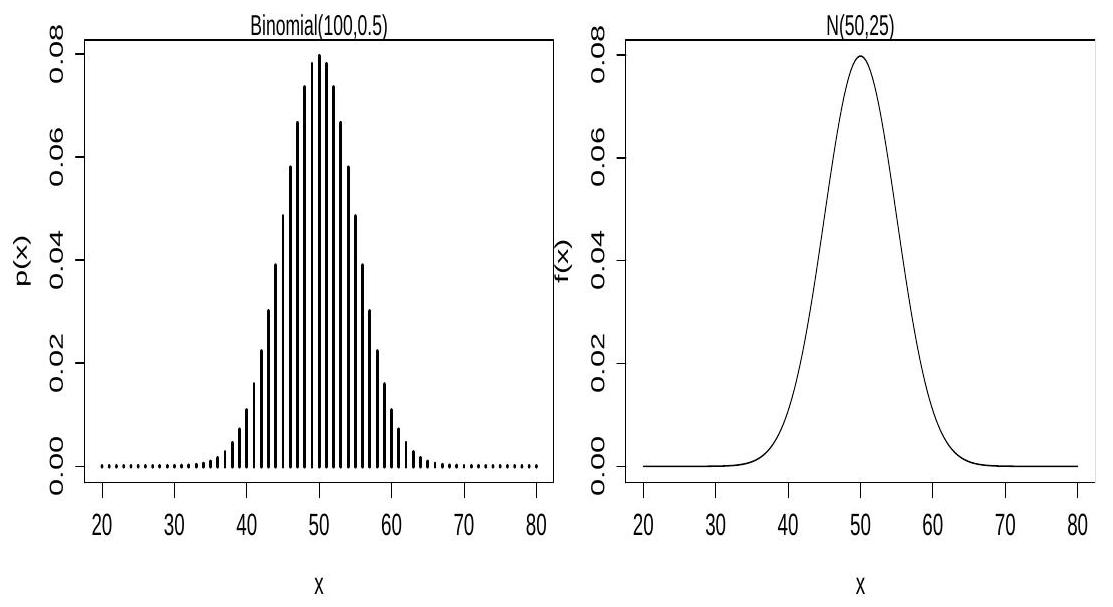
\includegraphics[max width=\textwidth]{2025_05_12_2c033a5f0417cd8b136fg-33}
\end{center}

\section*{Binomial $\left(1000, \frac{1}{2}\right)$ pmf \& N $(500,250)$ pdf}
\begin{center}
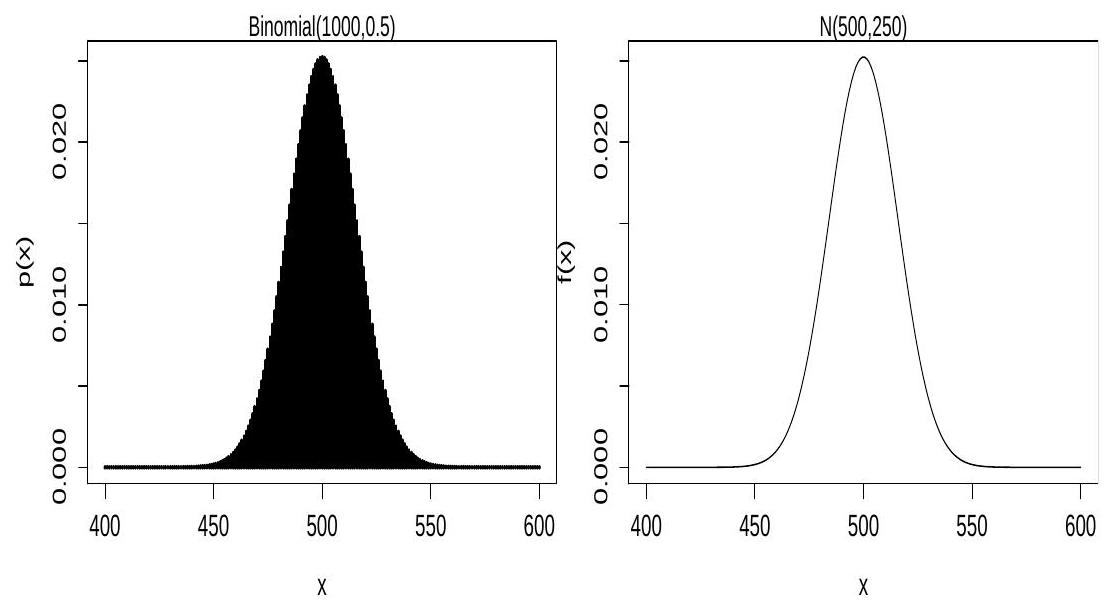
\includegraphics[max width=\textwidth]{2025_05_12_2c033a5f0417cd8b136fg-34}
\end{center}

\section*{Hypothesis Testing}
\section*{Motivation}
Suppose a video streaming company has developed a new feature for their tv app that they believe will increase user engagement. Before rolling it out to all users, they decide to conduct a so-called A/B test.\\

\includegraphics[max width=\textwidth, center]{2025_05_12_2c033a5f0417cd8b136fg-36}

A group of users (control group) will continue to use the current version of the app without the new feature, while another group (test group) will use the version of the app with the new feature.

\section*{Hypothesis Testing}
\begin{itemize}
  \item Consider the following two hypotheses:
  \item The Null Hypothesis: there is no difference in user engagement between the two groups.
  \item The Alternative Hypothesis: a difference exists, e.g., the new feature increases user engagement.
  \item If the test group shows much higher engagement than the control group, then we will reject the null hypothesis and conclude that the evidence favours the alternative hypothesis.
  \item This is an example of hypothesis testing. The idea is to assess the strength of the evidence in the sample data by which we can reject (or retain) the null hypothesis.
\end{itemize}

\section*{Parametric tests}
\begin{itemize}
  \item Suppose again we have a random i.i.d. sample $\left(X_{1}, \ldots, X_{n}\right)$ of a random variable $X$ from an unknown distribution $P$.
  \item Parametric tests typically assume the sample comes from a parametric family $P(\cdot \mid \theta)$ and test whether we could reasonably assume $\theta=\theta_{0}$ for some particular value $\theta_{0}$.
  \item In the $\mathrm{A} / \mathrm{B}$ testing example, we may set $X$ as the difference in user engagement feedbacks in the two groups and test if $\mu=0$ under the assumption that $X \sim \mathcal{N}\left(\mu, \sigma^{2}\right)$.
\end{itemize}

\section*{Hypotheses}
\begin{itemize}
  \item Formally, let $H_{0}$ be the null hypothesis and $H_{1}$ be the alternative hypothesis.
  \item Most often we simply test
\end{itemize}

$$
H_{0}: \theta=\theta_{0} \quad \text { versus } \quad H_{1}: \theta \neq \theta_{0} .
$$

This is known as a two-sided test.

\begin{itemize}
  \item A one-sided test is also possible, e.g.:
\end{itemize}

$$
\begin{array}{lll}
H_{0}: \theta=\theta_{0} \quad \text { versus } & H_{1}: \theta<\theta_{0} \\
H_{0}: \theta=\theta_{0} \quad \text { versus } & H_{1}: \theta>\theta_{0}
\end{array}
$$

\begin{itemize}
  \item Usually, the null hypothesis is formulated with an equality sign $(=)$, while the alternative hypothesis uses one of $(\neq,<,>)$.
\end{itemize}

\section*{Rejection Region for a Test Statistic}
\begin{itemize}
  \item To test the validity of $H_{0}$, we choose a test statistic $T(X)$ of the data for which we can find the distribution under $H_{0}$.
  \item The "art" of hypothesis testing is to define the test by identifying a rejection region $R \subseteq \mathbb{R}$ of low probability values of $T$ under the assumption that $H_{0}$ is true, so that
\end{itemize}

$$
P\left(T \in R \mid H_{0}\right)=\alpha
$$

for some small probability $\alpha$ (say $5 \%$ ). We call $\alpha$ the significance level of the test.

\begin{itemize}
  \item Rule: A well chosen rejection region will have relatively high probability under $H_{1}$, whilst retaining low probability under $H_{0}$.
  \item We calculate the observed test statistic $t(x)$ for our sample $x$ :\\
(1) If $t \in R$ we "reject the null hypothesis at the $100 \alpha \%$ level".\\
(2) If $t \notin R$ we "retain the null hypothesis at the $100 \alpha \%$ level".
\end{itemize}

\section*{Testing for Population Mean - Known Variance}
\begin{itemize}
  \item Suppose $X_{1}, \ldots, X_{n}$ are i.i.d. $N\left(\mu, \sigma^{2}\right)$ with only $\sigma^{2}$ known.
  \item We may wish to test if $\mu=\mu_{0}$ for some specific value $\mu_{0}$.
  \item Then we can state our null and alternative hypotheses as
\end{itemize}

$$
H_{0}: \mu=\mu_{0} \text { versus } H_{1}: \mu \neq \mu_{0}
$$

\begin{itemize}
  \item Under $H_{0}: \mu=\mu_{0}$, we then know both $\mu$ and $\sigma^{2}$. So for the sample mean $\bar{X}$ we know from the CLT that
\end{itemize}

$$
Z=\frac{\bar{X}-\mu_{0}}{\sigma / \sqrt{n}} \sim N(0,1)
$$

where $\sigma / \sqrt{n}$ is often called in statistics the standard error.

\begin{itemize}
  \item By the CLT, the result also holds approximately when the $X_{i}$ are not normally distributed.
\end{itemize}

\section*{Testing for Population Mean - Known Variance}
\begin{itemize}
  \item If the Z-test statistic takes "extreme" values far from zero, there is evidence to conclude that $H_{0}$ should be rejected. Otherwise, the data is inconclusive and we need to retain $H_{0}$.
  \item So we may define our rejection region $R$ to be the $100 \alpha \%$ tails of the standard normal distribution distribution,
\end{itemize}

$$
R=\left(-\infty,-z_{1-\frac{\alpha}{2}}\right) \cup\left(z_{1-\frac{\alpha}{2}}, \infty\right)
$$

we have $P\left(Z \in R \mid H_{0}\right)=\alpha$.

\begin{itemize}
  \item We thus reject $H_{0}$ at the $100 \alpha \%$ significance level exactly when our observed test statistic
\end{itemize}

$$
z=\frac{\bar{x}-\mu_{0}}{\sigma / \sqrt{n}} \in R
$$

\section*{Testing for Population Mean - Known Variance}
\begin{itemize}
  \item Rejection region $R$ for $z=\frac{\bar{x}-\mu_{0}}{\sigma / \sqrt{n}}$ at the $5 \%$ level:\\
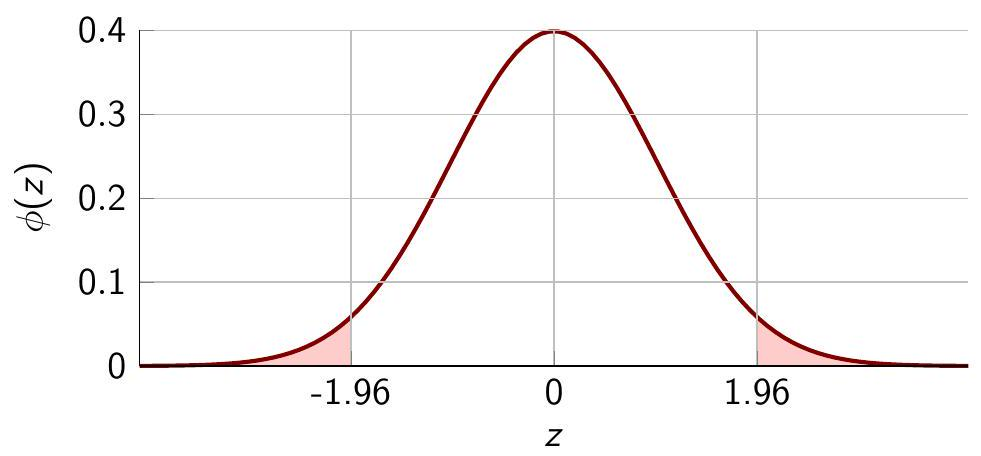
\includegraphics[max width=\textwidth, center]{2025_05_12_2c033a5f0417cd8b136fg-43}
  \item Each tail includes $\frac{\alpha}{2}=2.5 \%$ of the mass under $\phi(z)$.
\end{itemize}

\section*{Dealing with unknown variance}
\begin{itemize}
  \item As we measure a population (simulated or real), we may not know the real variance $\sigma^{2}$, but only the (bias-corrected) sample variance $S^{2}$. How do the formulas change in this case?
  \item The problem was studied by William S. Gosset, who published a paper in 1908 under the pseudonym Student.
  \item The study introduced the Student's $t$ distribution, a generalization of the Normal distribution, widely used in particular for statistical analysis of small samples.
  \item This is the basis of the $\mathbf{t}$-test statistic.
\end{itemize}

\section*{Student's t distribution}
$t_{\nu}$ : Student's $t$ distribution with $\nu$ degrees of freedom.\\
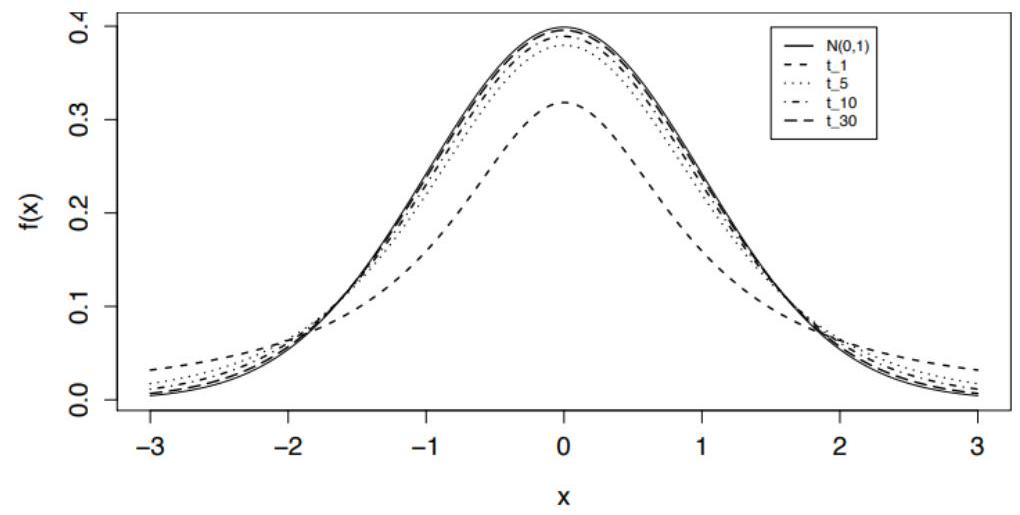
\includegraphics[max width=\textwidth, center]{2025_05_12_2c033a5f0417cd8b136fg-45}

\section*{Student's t distribution table}
Statistical table for the $p$-quantiles $t_{\nu, p}$ of the Student's $t$ distribution with $\nu$ degrees of freedom:

\begin{center}
\begin{tabular}{|l|l|l|l|l|l|l|l|l|l|}
\hline
 & \multicolumn{4}{|c|}{quantile} &  & \multicolumn{4}{|c|}{quantile} \\
\hline
$\nu$ & 0.95 & 0.975 & 0.99 & 0.995 & $\nu$ & 0.95 & 0.975 & 0.99 & 0.995 \\
\hline
1 & 6.31 & 12.71 & 31.82 & 63.66 & 9 & 1.83 & 2.26 & 2.82 & 3.25 \\
\hline
2 & 2.92 & 4.30 & 6.96 & 9.92 & 10 & 1.81 & 2.23 & 2.76 & 3.17 \\
\hline
3 & 2.35 & 3.18 & 4.54 & 5.84 & 12 & 1.78 & 2.18 & 2.68 & 3.05 \\
\hline
4 & 2.13 & 2.78 & 3.75 & 4.60 & 15 & 1.75 & 2.13 & 2.60 & 2.95 \\
\hline
5 & 2.02 & 2.57 & 3.36 & 4.03 & 20 & 1.72 & 2.09 & 2.53 & 2.85 \\
\hline
6 & 1.94 & 2.45 & 3.14 & 3.71 & 25 & 1.71 & 2.06 & 2.48 & 2.78 \\
\hline
7 & 1.89 & 2.36 & 3.00 & 3.50 & 40 & 1.68 & 2.02 & 2.42 & 2.70 \\
\hline
8 & 1.86 & 2.31 & 2.90 & 3.36 & $\infty$ & 1.645 & 1.96 & 2.326 & 2.576 \\
\hline
\end{tabular}
\end{center}

\section*{Testing for Population Mean - Unknown Variance}
\begin{itemize}
  \item If $\sigma^{2}$ in the previous example were unknown, we would have
\end{itemize}

$$
T=\frac{\bar{X}-\mu_{0}}{S / \sqrt{n}} \sim t_{n-1}
$$

which uses the Student's $t$ distribution with $n-1$ degrees of freedom ( $t_{n-1}$ ) and the bias-corrected sample std. dev. $S$.

\begin{itemize}
  \item So for a test of
\end{itemize}

$$
H_{0}: \mu=\mu_{0} \text { versus } H_{1}: \mu \neq \mu_{0}
$$

at the $\alpha$ level, the rejection region of our observed test statistic

$$
t=\frac{\bar{x}-\mu_{0}}{s / \sqrt{n}}
$$

is then given by $R=\left(-\infty,-t_{n-1,1-\frac{\alpha}{2}}\right) \cup\left(t_{n-1,1-\frac{\alpha}{2}}, \infty\right)$

\section*{Testing for Population Mean - Unknown Variance}
\begin{itemize}
  \item Rejection region $R$ for $n=6$ and $t=\frac{\bar{x}-\mu_{0}}{s / \sqrt{6}}$ at the $5 \%$ level:\\
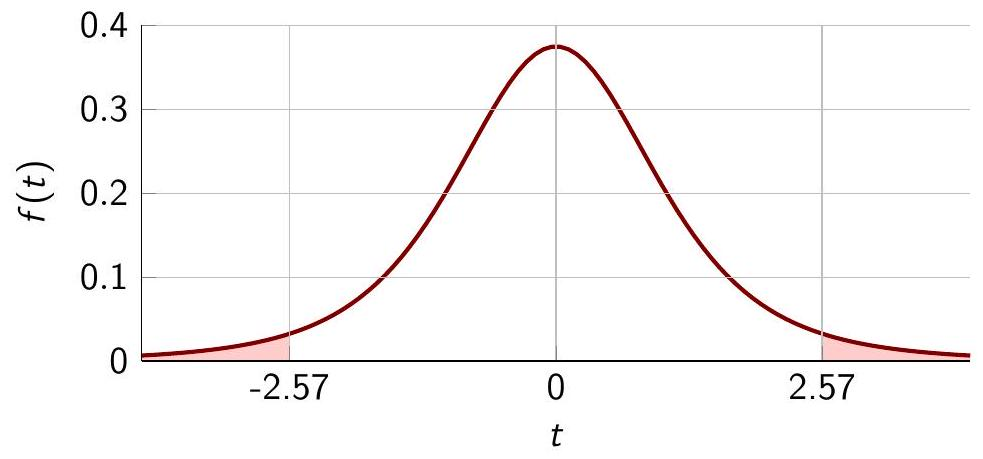
\includegraphics[max width=\textwidth, center]{2025_05_12_2c033a5f0417cd8b136fg-48}
\end{itemize}

\section*{p-Values}
\begin{itemize}
  \item Often, it is important to quantify the statistical significance of a result, in addition to giving a reject/retain outcome.
  \item The $\mathbf{p}$-value of the data is the probability of obtaining a test statistic at least as extreme as the one actually observed, assuming $H_{0}$ is correct.
  \item In other words, the p -value is the maximum significance level at which we still reject the null hypothesis $H_{0}$ for that sample.
  \item Thus, if we are given a fixed $\alpha$, the null hypothesis $H_{0}$ is rejected if the $p$-value is less than or equal to $\alpha$.
  \item Rule: Smaller $p$-values suggest stronger evidence against $H_{0}$.
\end{itemize}

\section*{$p$-Value in a One-sided Lower-Tailed Test ( $H_{1}: \theta<\theta_{0}$ )}
\begin{itemize}
  \item With known variance, the $p$-value is $\Phi(z)$.
  \item With unknown variance, the $p$-value is $F(t)$, where $F(\cdot)$ is the cdf of the Student's $t$ distribution.\\
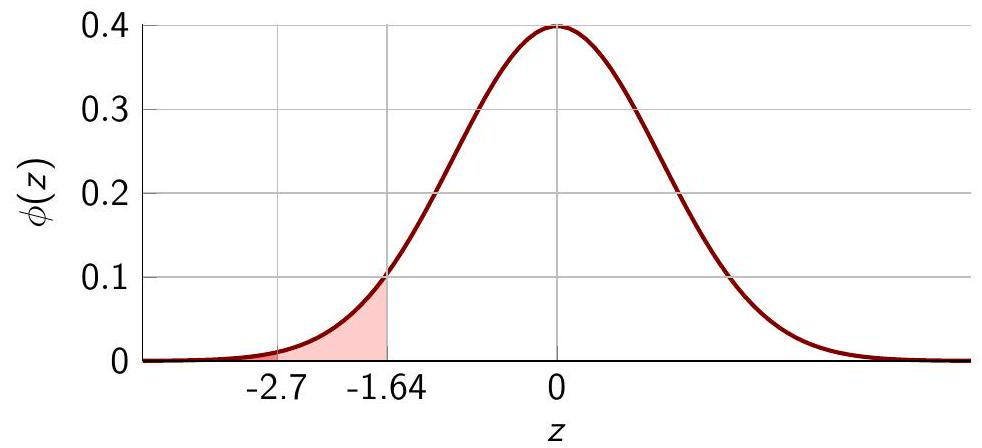
\includegraphics[max width=\textwidth, center]{2025_05_12_2c033a5f0417cd8b136fg-50}\\
$z=-2.7$ and $H_{1}: \theta<\theta_{0}$ then $p=0.003467$. The lighter shading is $R$ for $\alpha=0.05$.
\end{itemize}

\section*{$p$-Value in a One-sided Upper-Tailed Test ( $H_{1}: \theta>\theta_{0}$ )}
\begin{itemize}
  \item With known variance, the $p$-value is $1-\Phi(z)$.
  \item With unknown variance, the $p$-value is $1-F(t)$.\\
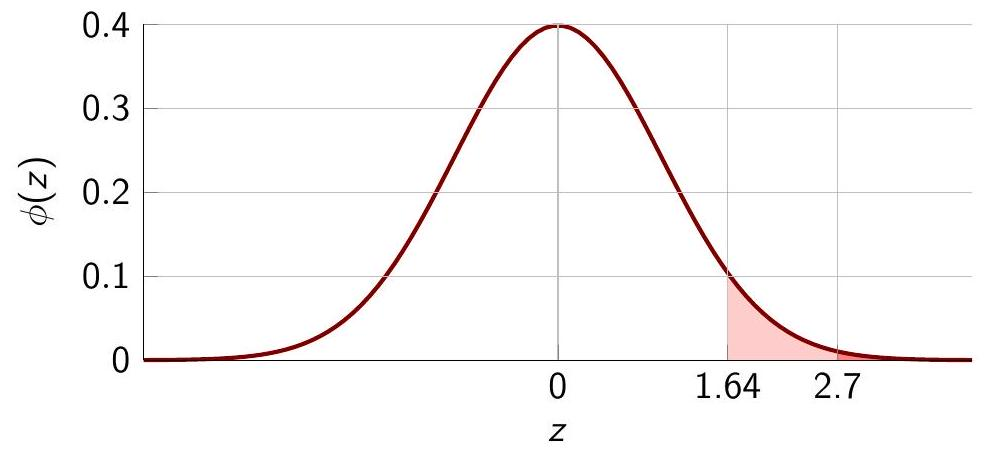
\includegraphics[max width=\textwidth, center]{2025_05_12_2c033a5f0417cd8b136fg-51}
\end{itemize}

If $z=2.7$ and $H_{1}: \theta>\theta_{0}$ then $p=0.003467$. The lighter shading is $R$ for $\alpha=0.05$.

\section*{$p$-Value in a Two-sided Test}
\begin{itemize}
  \item With known variance, the $p$-value is $2 \times(1-\Phi(|z|))$.
  \item With unknown variance, the $p$-value is $2 \times(1-F(|t|))$.\\
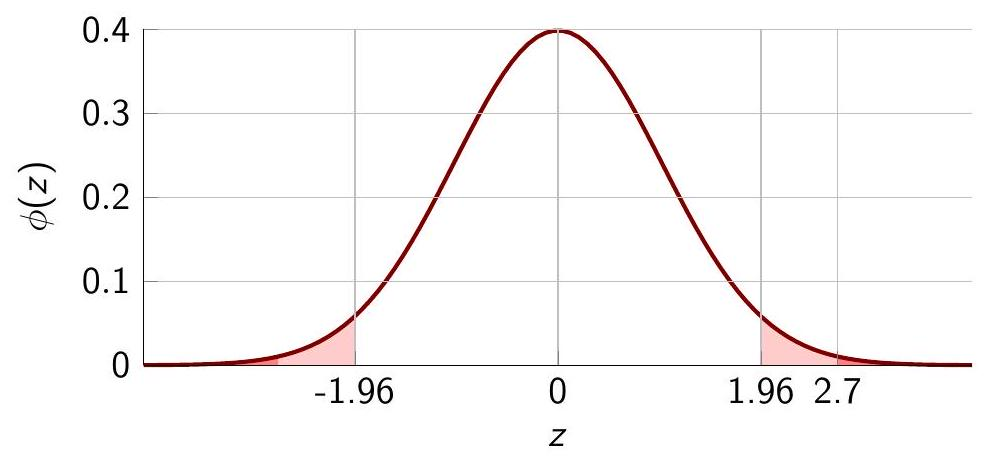
\includegraphics[max width=\textwidth, center]{2025_05_12_2c033a5f0417cd8b136fg-52}
\end{itemize}

For example, if $z=2.7$ then the two-sided $\mathbf{p}$-value is $p=0.006934$. The lighter shading is $R$ for $\alpha=0.05$.

\section*{Other commonly used tests (Unassessed)}
Besides the $Z$-test and the $t$-test, several other tests exist, e.g.:

\begin{itemize}
  \item Paired samples tests: Extensions exists of $Z$-test and $t$-test to compare samples in the form $\left(X_{1}, X_{1}^{\prime}\right), \ldots,\left(X_{n}, X_{n}^{\prime}\right)$.
  \item Chi-squared test: Used to assess whether observed frequencies of a random variable differ from expected.
  \item Kolmogorov-Smirnov test: Used to determine if two samples come from the same distribution or to compare a sample with a reference probability distribution.
\end{itemize}

\end{document}